\subsection{Definição dos modelos genéricos}
Com base no INI-C (2018) e no levantamento das edificações de escritório de Vitória, foram propostos dois tipos de modelos genéricos como base para o estudo das modificações de otimização e de produção de energia. Estes modelos representam os dois cenários de ambiente construído mais observados na cidade de Vitória. Estes cenários são formados por edificações mais baixas, com 8 pavimentos, e as mais altas, com 19 pavimentos. As dimensões utilizadas como referência para a construção dos modelos genéricos foram resultado dos valores médios observados nas edificações que compõe o levantamento.\vspace*{0.3cm} \newline
\noindent As características predominantes aplicadas aos modelos genéricos foram:
    \begin{itemize}\vspace*{-0.3cm}
        \item Número de pavimentos;\vspace*{-0.3cm}
        \item Forma - retangular;\vspace*{-0.3cm}
        \item Altura - gabarito e dimensões das fachadas;\vspace*{-0.3cm}
        \item Layout interno dos pavimento-tipo;\vspace*{-0.3cm}
        \item Ausência de proteção solar;\vspace*{-0.3cm}
        \item Percentual Total de Área de Abertura da Fachada.%\vspace*{-0.3cm}
    \end{itemize}
\noindent A composição dos modelos é baseada nas características predominantes e nos dados coletados \textit{in site}.%\vspace*{-0.5cm}
\subsubsection{Composição dos modelos genéricos}
A composição construtiva atribuída aos modelos utilizados neste trabalho mostra fundamentalmente os parâmetros necessários para a avaliação do desempenho energético segundo o INI-C. Os atributos utilizados serviram como ponto de partida para as análises subsequentes sugeridas nas etapas metodológicas e estão dispostos no Fluxograma da Figura \ref{fig:figura8}.\vspace{-0.10cm}%\pagebreak % disclaimer: não modificar pagebreak, pois é importante para manter a figura legível e as tabelas e elementos subsequentes nos seus devidos lugares.
    %\vspace*{-1cm}
    \begin{figure}[H]
        \centering
        \caption{Fatores utilizados como parâmetros de configuração volumétrica dos modelos genéricos.}
        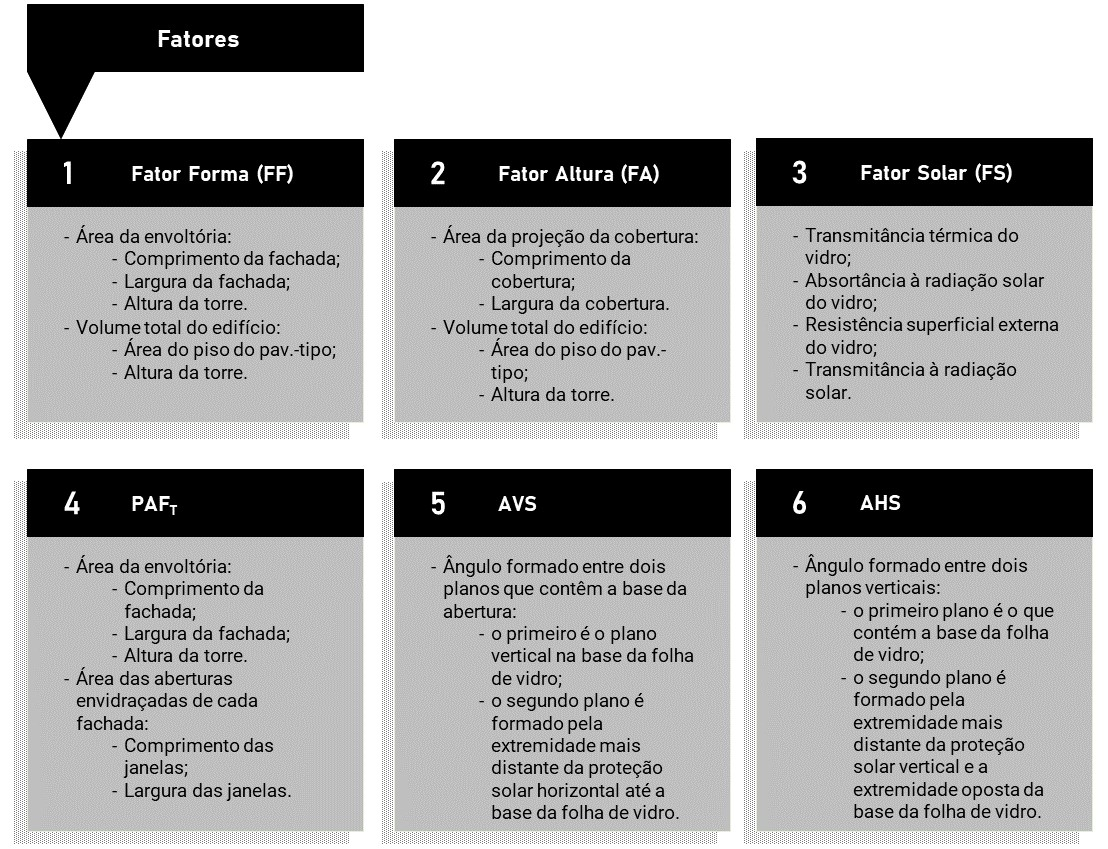
\includegraphics[width=0.9\textwidth]{figures/fig10_Fluxogramas-2.jpg}
        \begin{flushleft}
            \par \small Fonte: autor (2019)
        \end{flushleft}
        \label{fig:figura8}
    \end{figure}
\pagebreak
\noindent Apresentados na Tabela 7 e exemplificado na Figura \ref{fig:figura9}, os atributos estudados foram Fator de Forma, FF, Fator Altura, FA, Percentual de Área de Abertura da Fachada Total, PAFT, Ângulo Vertical de Sombreamento, AVS, e Ângulo Horizontal de Sombreamento, AHS.%\vspace*{0.3cm}
\begin{figure}[H]
    \centering
    \caption{Estrutura arquitetônica dos modelos genéricos.}
    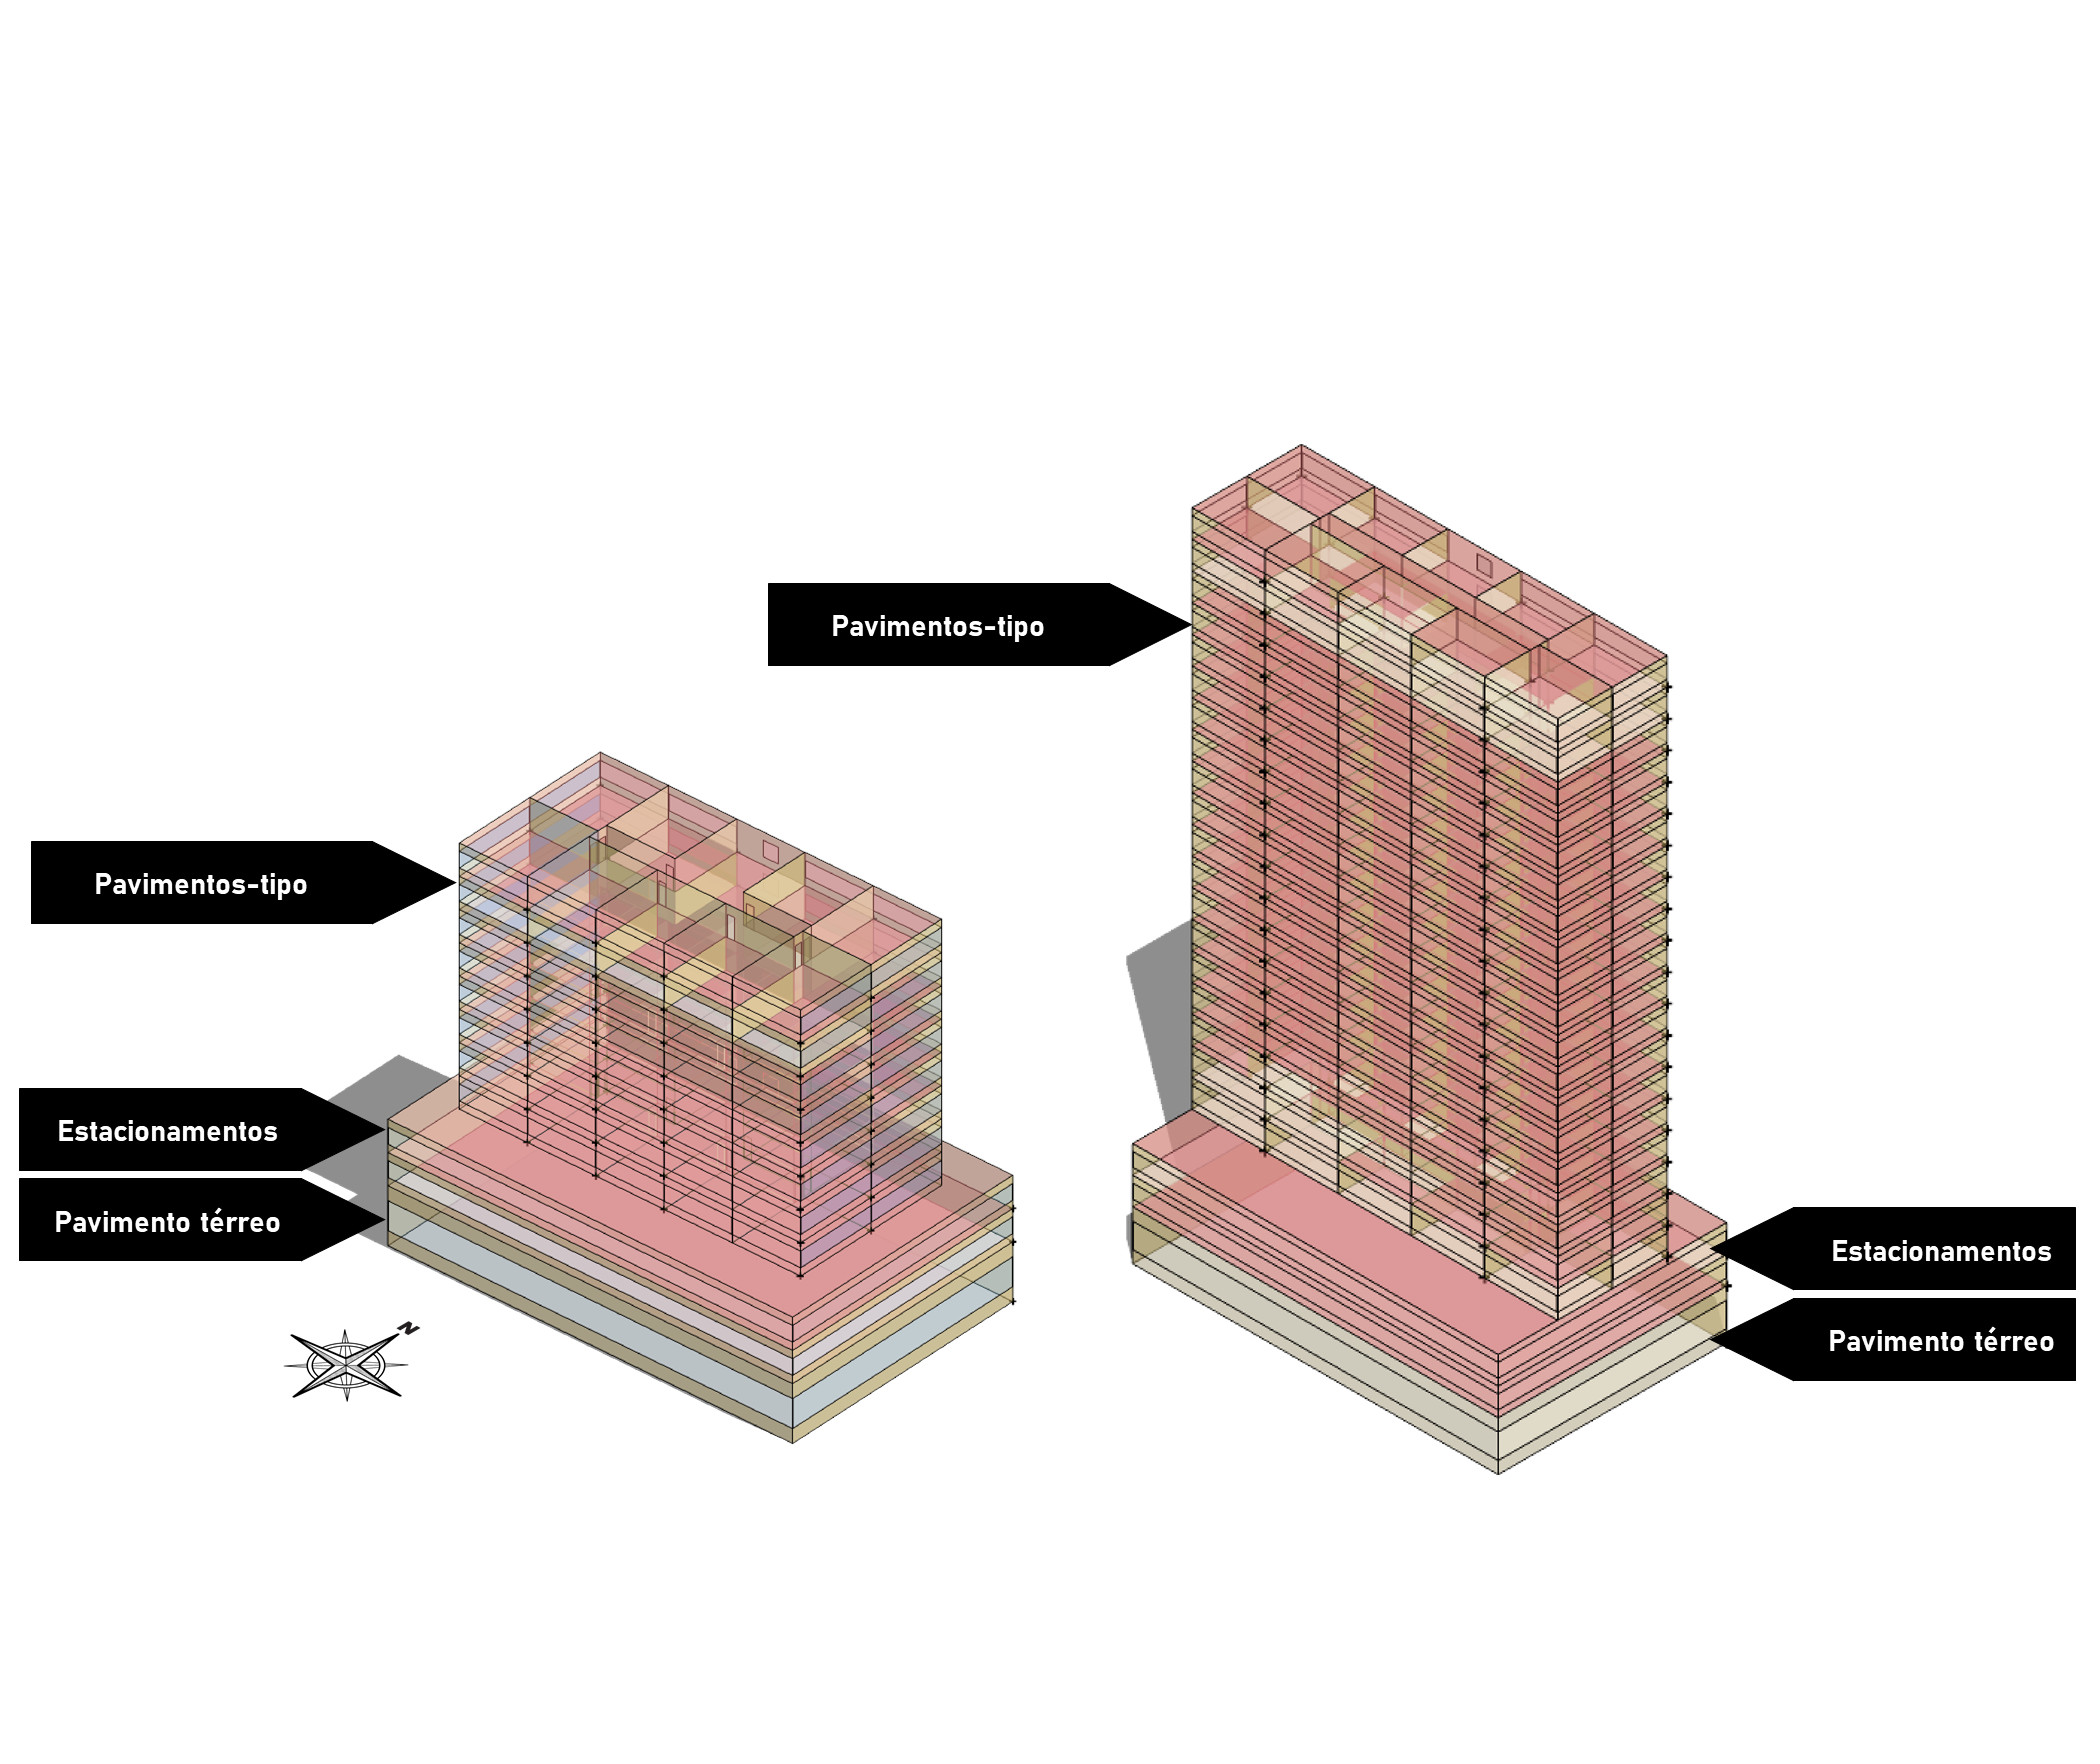
\includegraphics[width=0.9\textwidth]{figures/fig11_8-19-2pav.png}
    \begin{flushleft}
        \par \small Fonte: autor (2019).
    \end{flushleft}
    \label{fig:figura9}
\end{figure}
\noindent O PAF\textsubscript{T} e as propriedades do vidro utilizados para os modelos genéricos, como Fator Solar – FS, ou Solar Heat Gain Coefficient – SHGC, foram adotados considerando as médias desses atributos coletados in loco e complementados por dados extraídos do Catálogo de Propriedades Térmicas e Óticas de Vidro \cite{CentroBrasileirodeEficienciaEnergeticaemEdificacoesCB3E2015,AssociacaoBrasileiradeNormasTecnicas-ABNT2003}, da NBR 15220 (2003) e do INI-C \cite{InstitutoNacionaldeMetrologiaNormalizacaoeQualidadeIndustrial-INMETRO2018}, como forma de tornar genéricos os dados empregados, como apresentado na Tabela \ref{tab:tabela8}.%\vspace*{0.3cm} \newline
\begin{table}[H]
    \centering
    \small
    \caption{Parâmetros arquitetônicos dos modelos genéricos.}
    \begin{tabular*}{\columnwidth}{@{\extracolsep{\fill}}l|ll}
    \hline
    \textbf{Parâmetro}                                                              & \textbf{Descrição}         & \textbf{Referências}  \\ \hline
    \multicolumn{3}{c}{\textbf{Dados dimensionais dos pavimentos-tipo}}\\\hline
    Número de pavimento (un)                                                        & 8                          & 19                    \\ \hline
    \makecell[l]{Proporção geométrica – pav.\\ tipo (m – Comprimento x Largura)}    & 33,75x16                   & 40x12                 \\ \hline
    Altura do pavimento-tipo (m)                                                    & 3                          & 3                     \\ \hline
    \makecell[l]{Área total construída – pavimentos-tipo (m²)}                      & 4.320                      & 9.120                 \\ \hline
    Área de projeção da cobertura - Apcob (m²)                                      & 843,75                     & 640,00                \\ \hline
    Área de projeção do edifício - Ape (m²)*                                        & 1000                       & 1000                  \\ \hline
    Área total construída - Atot (m²)                                               & 7.320                      & 12.120                \\ \hline
    Volume Total da Edificação - Vtot (m³)                                          & 24.360                     & 38.760                \\ \hline
    Área da envoltória - Aenv (m²)                                                  & 5.430,30                   & 8.890,00              \\ \hline
    Fator de Forma (FF)                                                             & 0,222                      & 0,229                 \\ \hline
    Fator Altura (FA)                                                               & 0,125                      & 0,052                 \\ \hline
    Fator Solar (FS)                                                                & 0,44                       & 0,44                  \\ \hline
    Transmitância do vidro (W/m²K)                                                  & 5,6                        & 5,6                   \\ \hline
    Área de aberturas das fachadas – Aabert (m²)                                    & 1.501,80                   & 3.152,40              \\ \hline
    PAF\textsubscript{T} (\%)                                                       & 50\%                       & 50\%                  \\ \hline
    \makecell[l]{Ângulo Vertical (AVS) e Horizontal\\ (AHS) de Sombreamento (°)}    & 0                          & 0                     \\ \hline
    \end{tabular*}
    \begin{flushleft}
        \par \small Fonte: autor (2019); *A Ape contempla a área de projeção do pavimento térreo e estacionamentos.\vspace{-0.35cm}
    \end{flushleft}
    \label{tab:tabela8}
\end{table}
\noindent Segundo o INI-C, publicado pelo \textcite{InstitutoNacionaldeMetrologiaNormalizacaoeQualidadeIndustrial-INMETRO2018}, a utilização do Ângulo de Obstrução Vertical – AOV, para a simulação de obstruções solares parciais e totais são critérios opcionais que dependem da condição real levantada. Apesar da obstrução solar lateral ter sido uma condição observada em algumas edificações de Vitória, com base na observação da frequência de ocorrência, este atributo não foi considerado para o presente trabalho dada a configuração e disposição das edificações do recorte territorial em relação ao lote, que possibilitaram utilizar cenários sem obstrução solar. Além disso, para o estudo da incidência de radiação solar sobre a edificação e como ponto de partida para a implementação das estratégias passivas aos modelos genéricos, foi definido a fachada principal com orientação Sul, de acordo com a frequência de ocorrência observada na amostragem.\pagebreak

\noindent O pavimento térreo e dois pavimentos de estacionamentos (Figura \ref{fig:figura10}), foram centralizados na base das torres em ambos os modelos, com dimensões idênticas e de forma genérica, com o intuito de evidenciar a influência sobre o consumo energético total por meio do número de pavimentos. Contudo, o uso e ocupação destas áreas se torna de baixa relevância, uma vez que as atividades de maior permanência se dão nos ambientes da torre.

\noindent Estes pavimentos compreendem características arquitetônicas apresentadas em todas as edificações selecionadas em levantamento. Posteriormente, na etapa de produção de energia, foi proposto o deslocamento dos pavimentos abaixo da torre para aproveitamento de área para inserção de painéis fotovoltaicos.
\begin{figure}[H]
    \centering
    \caption{Conformação do pavimento térreo e estacionamentos.}
    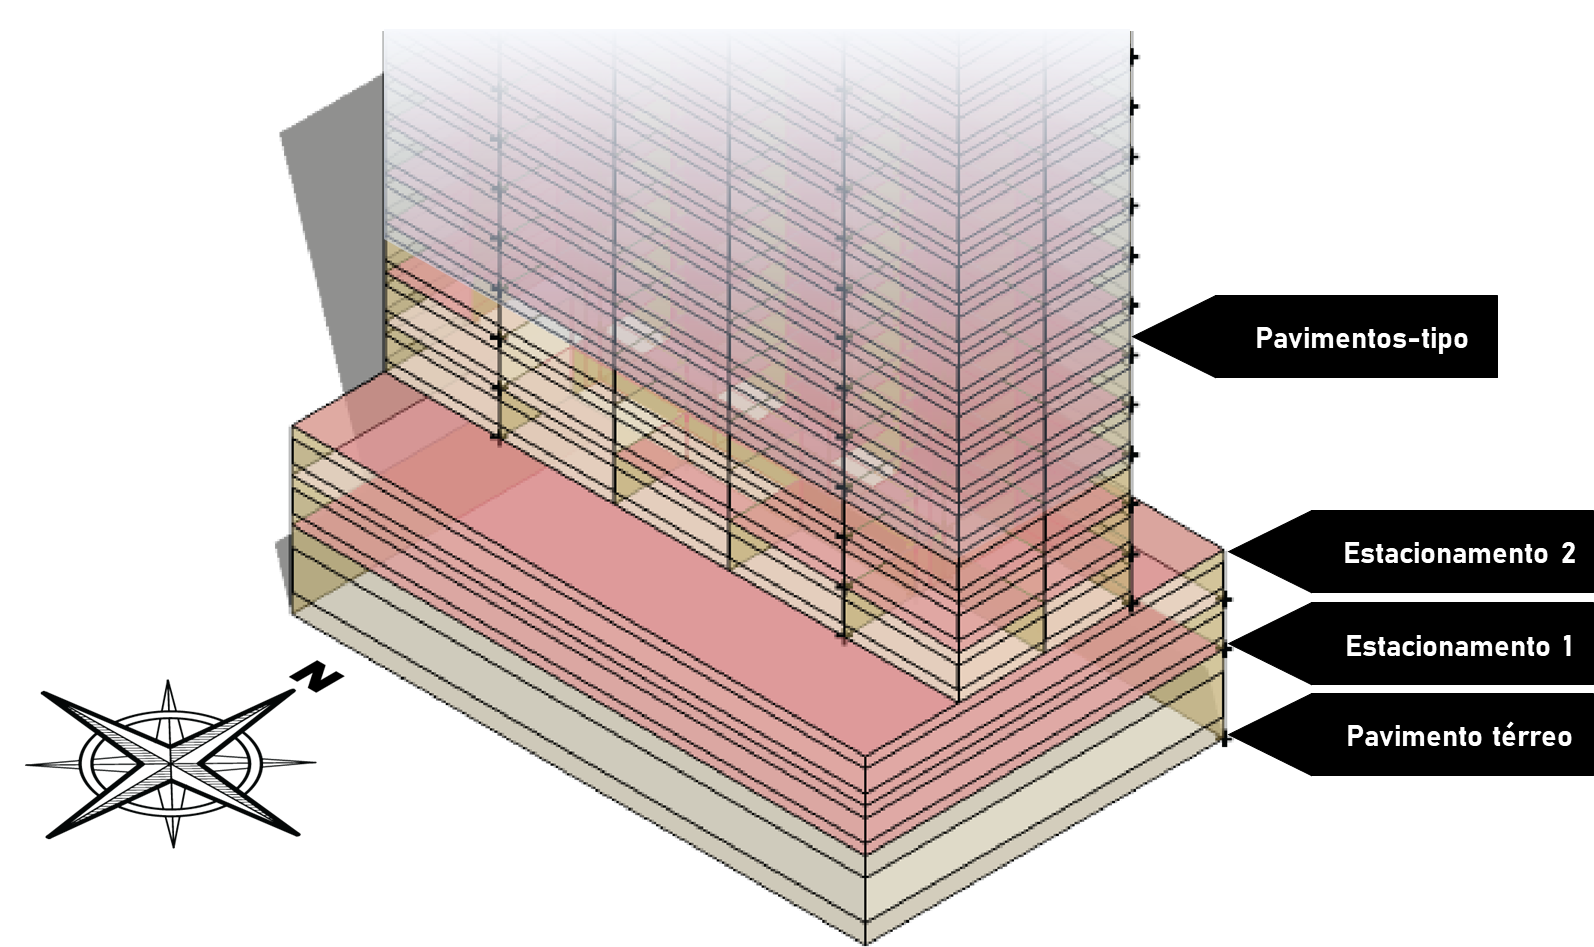
\includegraphics[width=0.9\textwidth]{figures/fig12-base_torre-1.png}
    \begin{flushleft}
        \par \small Fonte: autor (2019).
    \end{flushleft}
    \label{fig:figura10}
\end{figure}\vspace*{-0.5cm}
\noindent Os modelos são distinguidos principalmente pela área de projeção, número de pavimentos, pelo volume total e área da envoltória. Esses fatores resultam diretamente em Fator de Forma e Fator Altura distintos para cada modelo, amparando um dos objetivos específicos desta pesquisa sobre identificar as características mais influentes no consumo de energia elétrica. As zonas térmicas também formam características distintas entre os modelos genéricos, variando as áreas úteis, como apresentado na Tabela \ref{tab:tabela9}.
\begin{table}[H]
    \centering
    \small
    \caption{Zonas térmicas dos modelos genéricos.}
    \begin{tabular*}{\columnwidth}{@{\extracolsep{\fill}}ll}\hline
        \makecell[c]{Zonas térmicas - modelo\\ genérico de 8 pavimentos}                    & \makecell[c]{Zonas térmicas - modelo \\genérico de 19 pavimentos}                 \\ \hline
        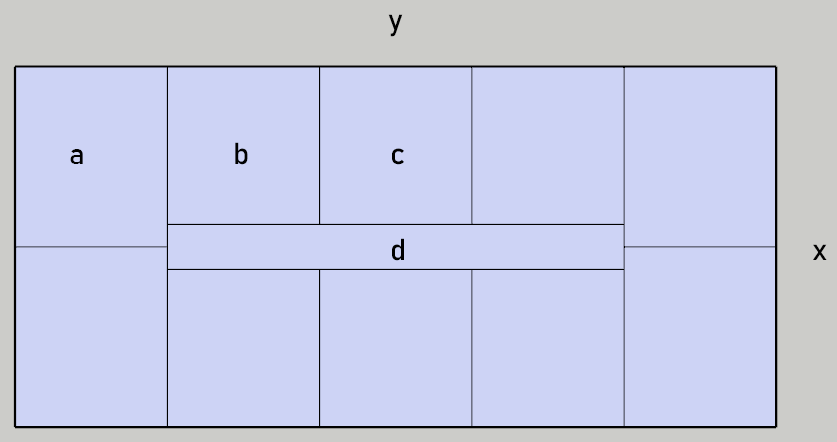
\includegraphics[width=0.5\textwidth]{figures/tab9-pb-8pav.png}                     & 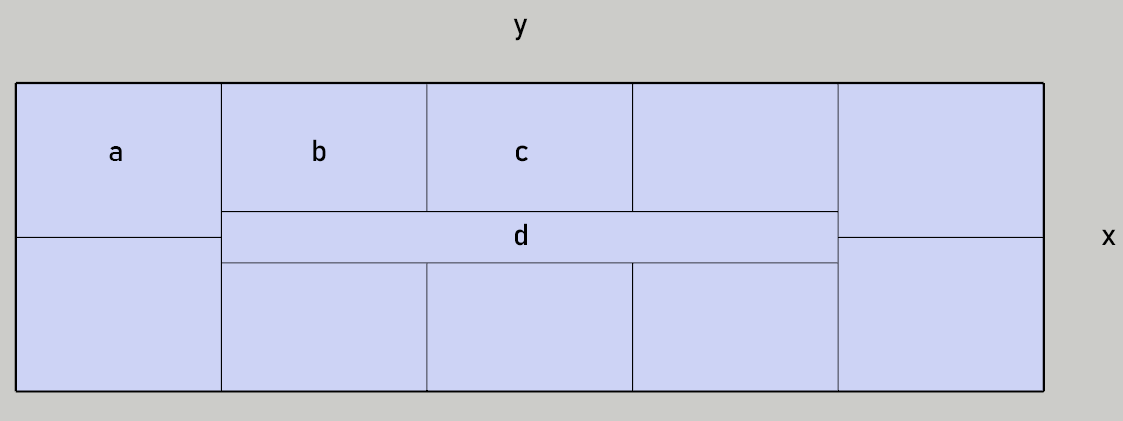
\includegraphics[width=0.5\textwidth]{figures/tab9-pb-19pav.png}                  \\
        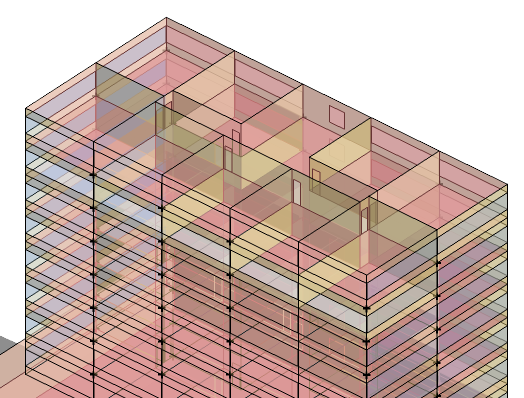
\includegraphics[width=0.5\textwidth]{figures/tab9-CEP_8pav-v3-7.png}               & 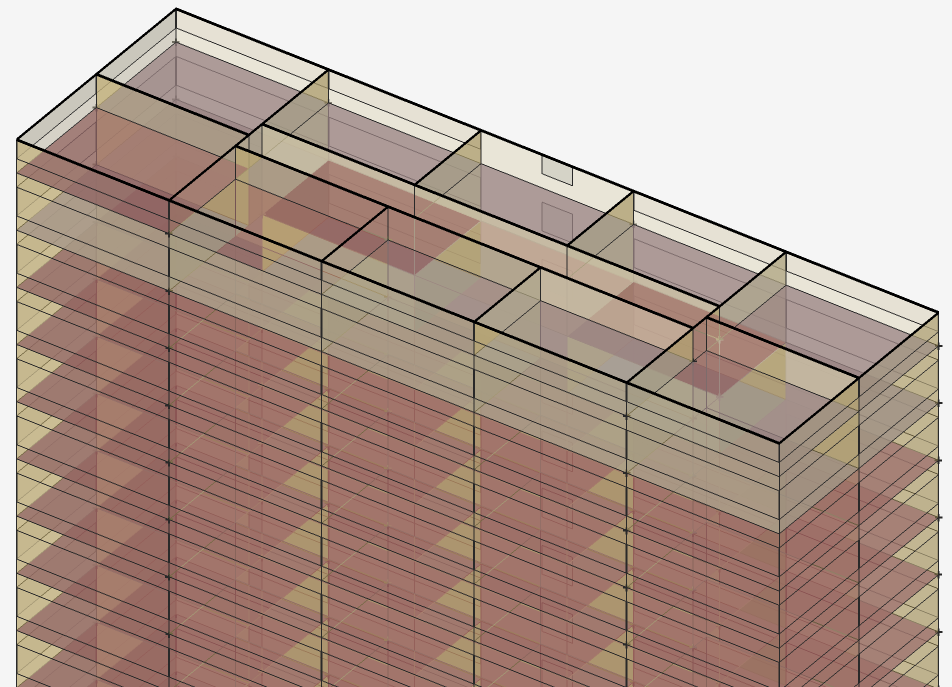
\includegraphics[width=0.5\textwidth]{figures/tab9-corte-19pav-v1.png}            \\ \hline
        Quantidade de zonas: 11                                                             & Quantidade de zonas: 11                                                           \\ \hline
        Área de projeção da torre: 843,75 m²                                                & Área de projeção da torre: 640,00 m²                                              \\ \hline
        Área da zona térmica “a”: 54,00 m²                                                  & Área da zona térmica “a”: 48,00 m²                                                \\ \hline
        Área da zona térmica “b”: 47,25 m²                                                  & Área da zona térmica “b”: 40,00 m²                                                \\ \hline
        Área da zona térmica “c+d”: 87,75 m²                                                & Área da zona térmica “c+d”: 88,00 m²                                              \\ \hline
        \makecell[l]{Largura do pavimento-tipo\\ (x): 16,00 m}                              & Largura do pavimento-tipo (x): 12,00 m                                            \\ \hline
        \makecell[l]{Comprimento do pavimento-\\tipo (y): 33,75 m}                          & \makecell[l]{Comprimento do pavimento-\\tipo (y): 40,00 m}                        \\ \hline
        \makecell[l]{Dimensões das aberturas\\ das zonas térmicas – N/S:\\ 6,70x1,51 m}     & \makecell[l]{Dimensões das aberturas das zonas\\ térmicas – N/S: 7,95x1,51 m}     \\ \hline
        \makecell[l]{Dimensões das aberturas\\ das zonas térmicas – L/O:\\ 7,95x1,51 m}     & \makecell[l]{Dimensões das aberturas das zonas\\ térmicas – L/O: 5,95x1,51 m}     \\ \hline
        \makecell[l]{Dimensões das aberturas\\ das zonas térmicas – circ.:\\ 1,49x1,51 m}   & \makecell[l]{Dimensões das aberturas das zonas\\ térmicas – circ.: 1,49x1,51 m}   \\ \hline
        \multicolumn{2}{l}{Dimensões das zonas térmicas – Pav. térreo e garagens: 40 x 25 m}                                                                                    \\ \hline
        \multicolumn{2}{l}{\makecell[l]{Dimensões das aberturas das zonas térmicas – Pav.\\ térreo e gar.: 39,95x1,51 m (N/S); 24,95x1,51 m (L/O)}}                             \\ \hline
    \end{tabular*}
    \begin{flushleft}
        \par \small Fonte: autor (2019).
    \end{flushleft}
    \label{tab:tabela9}
\end{table}
\pagebreak

\noindent Foram propostas, na etapa de otimização, proteções solares horizontais para as aberturas, que servem como proteção à radiação solar direta e controle de iluminação natural em horários predeterminados – 9, 12 e 15 horas. Este controle de horários de incidência solar se deu pelo comprimento das proteções solares propostas. Esta solução foi adotada como estratégia passiva. Utilizou-se, também, a área para proteção solar como espaço para exploração de energia solar por meio de painéis fotovoltaicos sobre os elementos protetores, como exemplificado na Figura \ref{fig:figura11} \cite{Didone2014a}.
\begin{figure}[H]
    \centering
    \caption{Painéis fotovoltaicos sobre as proteções solares da fachada oeste e cobertura.}
    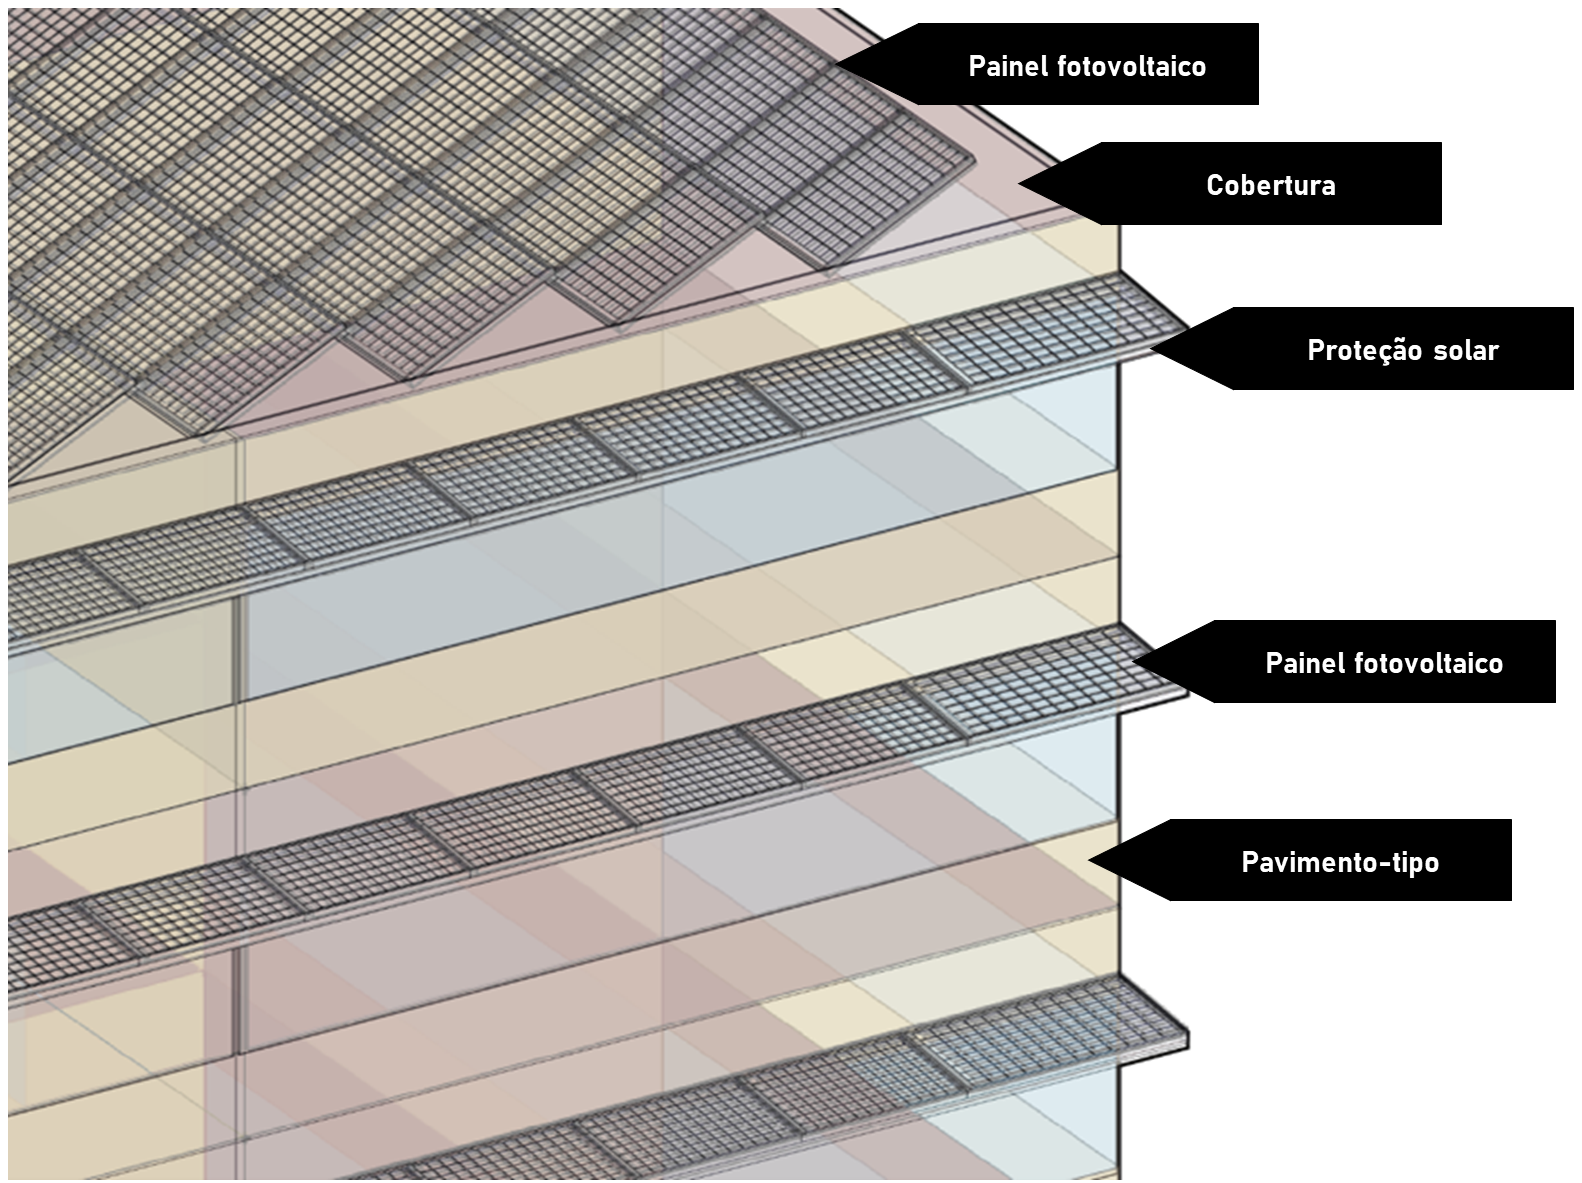
\includegraphics[width=0.9\textwidth]{figures/fig13-paineis pv.png}
    \begin{flushleft}
        \par \small Fonte: autor (2019).
    \end{flushleft}
    \label{fig:figura11}
\end{figure}
\subsubsection{Parâmetros arquitetônicos dos modelos genéricos}
\noindent A preparação para o início das simulações é precedida pela definição dos parâmetros arquitetônicos e das variáveis contidas em cada um destes. Com base no levantamento in loco e no referencial teórico, são inicialmente modificados os atributos arquitetônicos em três fases: envoltória, sistemas de iluminação e condicionamento de ar. As modificações foram implementadas de forma ordenada, a fim de evidenciar a influência de cada medida proposta no consumo final de energia elétrica da edificação genérica. As medidas propostas para analise por meio de simulação computacional estão apresentadas na Tabela \ref{tab:tabela10}.
\begin{table}[H]
    \small
    \caption{Zonas térmicas dos modelos genéricos.}%\vspace*{0.3cm}
    \label{tab:tabela10}
    \begin{tabular*}{\columnwidth}{@{\extracolsep{\fill}}clcrl}
    \hline
    \multicolumn{2}{c}{Parâmetros}                                                                                                                      & \multicolumn{2}{c}{Variáveis} & Descrição                                                                                                                                                                                                                                                                                                                                                                                                                                                                 \\ \hline
    \multicolumn{1}{c}{\multirow{4}{*}{1}} & \multirow{4}{*}{Orientação Solar}                                                                          & a          & 0°               & \multirow{4}{*}{\makecell[l]{Orientação solar da fachada \\principal.}}                                                                                                                                                                                                                                                                                                                                                                                                   \\
    \multicolumn{1}{c}{}                   &                                                                                                            & b          & 90º              &                                                                                                                                                                                                                                                                                                                                                                                                                                                                           \\
    \multicolumn{1}{c}{}                   &                                                                                                            & c          & 180º             &                                                                                                                                                                                                                                                                                                                                                                                                                                                                           \\
    \multicolumn{1}{c}{}                   &                                                                                                            & d          & 270º             &                                                                                                                                                                                                                                                                                                                                                                                                                                                                           \\ \hline
    \multirow{8}{*}{2}                     & \multirow{8}{*}{Vidro com baixo Fator Solar}                                                               &            &                  & \multirow{8}{*}{\makecell[l]{Foram simuladas duas \\situações aplicas aos modelos \\genéricos: a primeira utilizando \\o vidro levantado in loco \\(a) e o modelo mais eficiente \\comercializado no mercado \\brasileiro (b) (CB3E; \\ABIVIDRO, 2015).}}                                                                                                                                                                                                                   \\
                                           &                                                                                                            &            &                  &                                                                                                                                                                                                                                                                                                                                                                                                                                                                           \\
                                           &                                                                                                            & a          & FS: 0,44         &                                                                                                                                                                                                                                                                                                                                                                                                                                                                           \\
                                           &                                                                                                            &            &                  &                                                                                                                                                                                                                                                                                                                                                                                                                                                                           \\
                                           &                                                                                                            &            &                  &                                                                                                                                                                                                                                                                                                                                                                                                                                                                           \\
                                           &                                                                                                            & b          & FS: 0,16         &                                                                                                                                                                                                                                                                                                                                                                                                                                                                           \\
                                           &                                                                                                            &            &                  &                                                                                                                                                                                                                                                                                                                                                                                                                                                                           \\
                                           &                                                                                                            &            &                  &                                                                                                                                                                                                                                                                                                                                                                                                                                                                           \\ \hline
    \multirow{13}{*}{3}                    & \multirow{13}{*}{\makecell[l]{Percentual de Área de Abertura\\ da Fachada Total – PAF\textsubscript{T}}}   &            &                  & \multirow{13}{*}{\makecell[l]{As aberturas das fachadas foram \\definidas de acordo com as \\indicações de programas de \\economia de energia como \\PROCEL EDIFICA e o \textit{Advanced} \\ \textit{Energy Design Guide for Small} \\ \textit{to Medium Office Buildings} \\(Guia Avançado de Planejamento \\Energético para Edificações de \\Escritório de Pequeno e Médio \\Porte) da ASHRAE (ASHRAE \\et al., 2014, 2019; FERRADOR \\FILHO; AGUIAR; KNIESS, 2018).}}  \\
                                           &                                                                                                            &            &                  &                                                                                                                                                                                                                                                                                                                                                                                                                                                                           \\
                                           &                                                                                                            &            &                  &                                                                                                                                                                                                                                                                                                                                                                                                                                                                           \\
                                           &                                                                                                            & a          & 30\%             &                                                                                                                                                                                                                                                                                                                                                                                                                                                                           \\
                                           &                                                                                                            &            &                  &                                                                                                                                                                                                                                                                                                                                                                                                                                                                           \\
                                           &                                                                                                            &            &                  &                                                                                                                                                                                                                                                                                                                                                                                                                                                                           \\
                                           &                                                                                                            & b          & 50\%             &                                                                                                                                                                                                                                                                                                                                                                                                                                                                           \\
                                           &                                                                                                            &            &                  &                                                                                                                                                                                                                                                                                                                                                                                                                                                                           \\
                                           &                                                                                                            &            &                  &                                                                                                                                                                                                                                                                                                                                                                                                                                                                           \\
                                           &                                                                                                            & c          & 80\%             &                                                                                                                                                                                                                                                                                                                                                                                                                                                                           \\
                                           &                                                                                                            &            &                  &                                                                                                                                                                                                                                                                                                                                                                                                                                                                           \\
                                           &                                                                                                            &            &                  &                                                                                                                                                                                                                                                                                                                                                                                                                                                                           \\
                                           &                                                                                                            &            &                  &                                                                                                                                                                                                                                                                                                                                                                                                                                                                           \\ \hline
    \multirow{8}{*}{4}                     & \multirow{8}{*}{\makecell[l]{Sistema de Condicionamento \\de Ar}}                                          &            &                  & \multirow{8}{*}{\makecell[l]{Foram adotados para a simulação \\o sistema de condicionamento de \\ar observado em levantamento, \\sendo este o Sistema Central de \\Água Gelada (CAG), o sistema \\individual \textit{Split}, e o \textit{Variable} \\ \textit{Refrigerant Fluid–VRF} \\(CBCS, 2015).}}                                                                                                                                                                    \\
                                           &                                                                                                            & a          & CAG/Fancoil      &                                                                                                                                                                                                                                                                                                                                                                                                                                                                           \\
                                           &                                                                                                            &            &                  &                                                                                                                                                                                                                                                                                                                                                                                                                                                                           \\
                                           &                                                                                                            & b          & Split            &                                                                                                                                                                                                                                                                                                                                                                                                                                                                           \\
                                           &                                                                                                            &            &                  &                                                                                                                                                                                                                                                                                                                                                                                                                                                                           \\
                                           &                                                                                                            & c          & VRF              &                                                                                                                                                                                                                                                                                                                                                                                                                                                                           \\
                                           &                                                                                                            &            &                  &                                                                                                                                                                                                                                                                                                                                                                                                                                                                           \\
                                           &                                                                                                            &            &                  &                                                                                                                                                                                                                                                                                                                                                                                                                                                                           \\ \hline
    \multirow{6}{*}{5}                     & \multirow{6}{*}{\makecell[l]{Transmitância térmica da \\parede da envoltória}}                             & a          & 2,46 W/m²K       & \multirow{6}{*}{\makecell[l]{Valores de transmitância \\baseados Anexo Geral V – Catálogo \\de Propriedades Térmicas de \\Paredes, Coberturas e Vidros \\(INMETRO, 2013).}}                                                                                                                                                                                                                                                                                               \\
                                           &                                                                                                            &            &                  &                                                                                                                                                                                                                                                                                                                                                                                                                                                                           \\
                                           &                                                                                                            & b          &                  &                                                                                                                                                                                                                                                                                                                                                                                                                                                                           \\
                                           &                                                                                                            &            & 0,38 W/m²K       &                                                                                                                                                                                                                                                                                                                                                                                                                                                                           \\
                                           &                                                                                                            &            &                  &                                                                                                                                                                                                                                                                                                                                                                                                                                                                           \\
                                           &                                                                                                            & c          & 0,32 W/m²K       &                                                                                                                                                                                                                                                                                                                                                                                                                                                                           \\ \hline
    \multirow{6}{*}{6}                     & \multirow{6}{*}{\makecell[l]{Transmitância térmica da \\cobertura}}                                        & a          & 3,73 W/m²K       & \multirow{6}{*}{\makecell[l]{Valores de transmitância \\baseados Anexo Geral V – Catálogo \\de Propriedades Térmicas de \\Paredes, Coberturas e Vidros \\(INMETRO, 2013).}}                                                                                                                                                                                                                                                                                               \\
                                           &                                                                                                            &            &                  &                                                                                                                                                                                                                                                                                                                                                                                                                                                                           \\
                                           &                                                                                                            & b          & 0,55 W/m²K       &                                                                                                                                                                                                                                                                                                                                                                                                                                                                           \\
                                           &                                                                                                            &            &                  &                                                                                                                                                                                                                                                                                                                                                                                                                                                                           \\
                                           &                                                                                                            &            &                  &                                                                                                                                                                                                                                                                                                                                                                                                                                                                           \\
                                           &                                                                                                            &            &                  &                                                                                                                                                                                                                                                                                                                                                                                                                                                                           \\ \hline
    \multicolumn{5}{c}{Continua}                                                                                                                                                                                                                                                                                                                                                                                                                                                                                                                                                                                                                                    \\ \hline
    \end{tabular*}
    \end{table} \pagebreak

    \begin{table}[H]
        \small
        \begin{tabular*}{\columnwidth}{@{\extracolsep{\fill}}clcrl}
        \hline
        \multicolumn{5}{c}{Conclusão}                                                                                                                                                                                                                                                                                                                                                                                                                                                                                                                                                                                                                                   \\ \hline
        \multicolumn{1}{c}{\multirow{5}{*}{7}} & \multirow{5}{*}{Proteção Solar}                                                                            &            &                  & \multirow{5}{*}{\makecell[l]{As proteções solares foram indicadas de acordo \\com a relação entre os horários de proteção e a \\incidência de luz solar nas salas avaliadas. \\O limite de dimensão destas proteções foi \\estabelecido segundo o Plano Diretor vigente.}}                                                                                                                                                                                                \\
        \multicolumn{1}{c}{}                   &                                                                                                            &            &                  &                                                                                                                                                                                                                                                                                                                                                                                                                                                                           \\
        \multicolumn{1}{c}{}                   &                                                                                                            &            &                  &                                                                                                                                                                                                                                                                                                                                                                                                                                                                           \\
        \multicolumn{1}{c}{}                   &                                                                                                            &            &                  &                                                                                                                                                                                                                                                                                                                                                                                                                                                                           \\
        \multicolumn{1}{c}{}                   &                                                                                                            &            &                  &                                                                                                                                                                                                                                                                                                                                                                                                                                                                           \\ \hline
        \multirow{7}{*}{8}                     & \multirow{7}{*}{\makecell[l]{Medidas de Redução de \\Carga de Energia Elétrica: \\Iluminação}}             &            &                  & \multirow{7}{*}{\makecell[l]{As medidas de redução de carga para ilumina-\\ção foram organizadas de acordo com as indi-\\cações do \textit{Advanced Energy Design Guide for} \\ \textit{Small to Medium Office Buildings} (Guia Avança-\\do de Planejamento Energético para Edificações \\de Escritório de Pequeno e Médio Porte) \\da ASHRAE (ASHRAE et al., 2019).}}                                                                                                     \\
                                               &                                                                                                            &            &                  &                                                                                                                                                                                                                                                                                                                                                                                                                                                                           \\
                                               &                                                                                                            & a          & FS: 0,44         &                                                                                                                                                                                                                                                                                                                                                                                                                                                                           \\
                                               &                                                                                                            &            &                  &                                                                                                                                                                                                                                                                                                                                                                                                                                                                           \\
                                               &                                                                                                            &            &                  &                                                                                                                                                                                                                                                                                                                                                                                                                                                                           \\
                                               &                                                                                                            &            &                  &                                                                                                                                                                                                                                                                                                                                                                                                                                                                           \\
                                               &                                                                                                            &            &                  &                                                                                                                                                                                                                                                                                                                                                                                                                                                                           \\ \hline
        \multirow{7}{*}{9}                     & \multirow{7}{*}{\makecell[l]{Medidas de Redução de \\Carga de Energia Elétrica: \\Equipamentos}}           &            &                  & \multirow{7}{*}{\makecell[l]{As medidas de redução de carga para equipa-\\mentos foram organizadas de acordo com as indi-\\cações do \textit{Advanced Energy Design Guide for} \\ \textit{Small to Medium Office Buildings} (Guia Avança-\\do de Planejamento Energético para Edificações \\de Escritório de Pequeno e Médio Porte) \\da ASHRAE (ASHRAE et al., 2019).}}                                                                                     \\
                                               &                                                                                                            &            &                  &                                                                                                                                                                                                                                                                                                                                                                                                                                                                           \\
                                               &                                                                                                            & a          & n/a              &                                                                                                                                                                                                                                                                                                                                                                                                                                                                           \\
                                               &                                                                                                            &            &                  &                                                                                                                                                                                                                                                                                                                                                                                                                                                                           \\
                                               &                                                                                                            &            &                  &                                                                                                                                                                                                                                                                                                                                                                                                                                                                           \\
                                               &                                                                                                            &            &                  &                                                                                                                                                                                                                                                                                                                                                                                                                                                                           \\
                                               &                                                                                                            &            &                  &                                                                                                                                                                                                                                                                                                                                                                                                                                                                           \\ \hline
        \end{tabular*}
        \begin{flushleft}
            \par \small Fonte: autor (2019).
        \end{flushleft}
        \end{table}
\vspace{-0.5cm} \noindent As variáveis de sistema de condicionamento de ar e medidas de redução de carga de energia elétrica foram adotadas como estratégias ativas de redução de consumo de energia. Dentre as variáveis, pode-se definir que:
\begin{itemize}
    \item O Sistema Central de Água Gelada – CAG, apresenta COP de referência de 2,93, entretanto, este parâmetro foi elevado para aproximadamente 5,00, com base no modelo padrão da ferramenta de simulação adotada e em modelos encontrados no mercado brasileiro. Esta modificação tem a finalidade de evidenciar a performance dos equipamentos propostos como substitutos aos sistemas utilizados nas edificações comerciais de escritório de Vitória. Desta forma, além do CAG, foram avaliados os sistemas VRF e Split, com configuração de COP de referência de 5,00;
    \item As medidas de redução de carga de energia elétrica têm por função aumentar a eficiência energética dos componentes dos sistemas de iluminação e equipamentos da edificação proposta. Estes critérios são recomendados por guias \cite{AmericanSocietyofHeatingRefrigeratingandAir-ConditioningEngineers-ASHRAE2019} e instruções normativas \cite{InstitutoNacionaldeMetrologiaNormalizacaoeQualidadeIndustrial-INMETRO2018a} voltadas à mitigação de consumo de energia.
\end{itemize}
\noindent As estratégias passivas foram aplicadas por meio da modificação dos aspectos construtivos como baixa transmitância térmica para vidros, paredes e cobertura, proteções solares sobre as aberturas da fachada e alteração do PAF\textsubscript{T}.
\noindent As alterações de paredes e cobertura propostas tem como objetivo reduzir a transmissão térmica de radiação solar entre ambientes e reduzir a carga térmica sobre o ultimo pavimento. Estas modificações são sugeridas para os componentes onde há maior área exposta à ação térmica do Sol. As propriedades das paredes e coberturas são apresentadas na Tabela \ref{tab:tabela11}.
\begin{table}[H]
    \small
    \caption{Propriedades físicas das paredes e coberturas propostas.}%\vspace*{0.3cm}
    \label{tab:tabela11}
    \begin{tabular}{lccl}
    \hline
    \multicolumn{4}{c}{\textbf{Paredes}}                                                                                                                                                                                                                                                                                                                                                                                    \\ \hline
    \makecell[c]{\textbf{Esquema} \\ \textbf{Volumétrico}}                          & \multicolumn{1}{c}{\makecell[c]{\textbf{Transmitância} \\ \textbf{térmica} \\ \textbf{W/(m²K)}}}   & \multicolumn{1}{c}{\makecell[c]{\textbf{Carga} \\ \textbf{térmica} \\ \textbf{(kJ/m²K)}}}  & \textbf{Descrição}                                                                                                                  \\ \hline
    \multirow{8}{*}{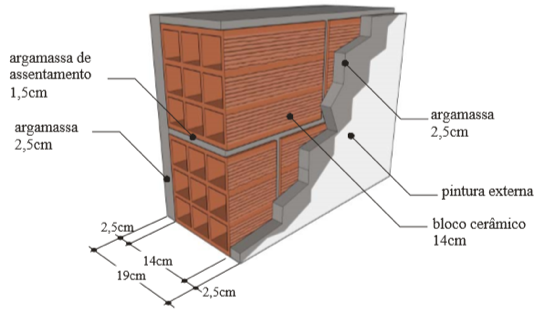
\includegraphics[width=0.4\textwidth]{figures/tab11-fig1.png}}  &                                                                       &                                                               & \multirow{8}{*}{\makecell[l]{Argamassa interna \\ \footnotesize(2,5cm); \\Bloco cerâmico \\ \footnotesize(14,0 x 19,0 x 29,0 cm);\\ Argamassa externa \\ \footnotesize(2,5cm); \\Pintura externa (\(\alpha\)).}}                  \\
                                                                                    &                                                                       &                                                               &                                                                                                                                                                                               \\
                                                                                    &                                                                       &                                                               &                                                                                                                                                                                               \\
                                                                                    &                                                                       &                                                               &                                                                                                                                                                                               \\
                                                                                    & 1,85                                                                  & 161                                                           &                                                                                                                                                                                               \\
                                                                                    &                                                                       &                                                               &                                                                                                                                                                                               \\
                                                                                    &                                                                       &                                                               &                                                                                                                                                                                               \\
                                                                                    &                                                                       &                                                               &                                                                                                                                                                                               \\ \hline
    \multirow{9}{*}{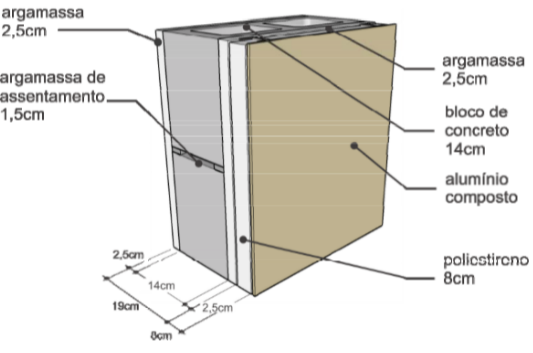
\includegraphics[width=0.4\textwidth]{figures/tab11-fig2.png}}  &                                                                       &                                                               & \multirow{9}{*}{\makecell[l]{Argamassa interna \\ \footnotesize(2,5 cm);\\ Bloco de concreto \\ \footnotesize(14,0 x 19,0 x 39,0 cm);\\ Argamassa externa \\ \footnotesize(2,5 cm);\\ Poliestireno \footnotesize(8 cm);\\ Placa de alumínio \\composto.}}  \\
                                                                                    &                                                                       &                                                               &                                                                                                                                                                                               \\
                                                                                    &                                                                       &                                                               &                                                                                                                                                                                               \\
                                                                                    &                                                                       &                                                               &                                                                                                                                                                                               \\
                                                                                    & 0,32                                                                  & 228                                                           &                                                                                                                                                                                               \\
                                                                                    &                                                                       &                                                               &                                                                                                                                                                                               \\
                                                                                    &                                                                       &                                                               &                                                                                                                                                                                               \\
                                                                                    &                                                                       &                                                               &                                                                                                                                                                                               \\
                                                                                    &                                                                       &                                                               &                                                                                                                                                                                               \\ \hline
    \multirow{9}{*}{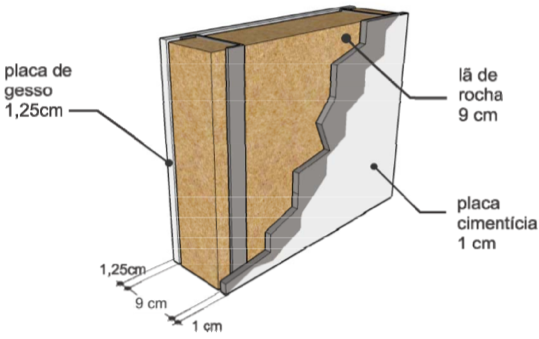
\includegraphics[width=0.4\textwidth]{figures/tab11-fig3.png}}  &                                                                       &                                                               & \multirow{9}{*}{\makecell[l]{Placa de gesso \\ \footnotesize(1,25 cm);\\ Lã de rocha \\ \footnotesize(9 cm);\\ Placa cimentícia \\ \footnotesize(1 cm).}}                                                                               \\
                                                                                    &                                                                       &                                                               &                                                                                                                                                                                               \\
                                                                                    &                                                                       &                                                               &                                                                                                                                                                                               \\
                                                                                    &                                                                       &                                                               &                                                                                                                                                                                               \\
                                                                                    & 0,38                                                                  & 269                                                           &                                                                                                                                                                                               \\
                                                                                    &                                                                       &                                                               &                                                                                                                                                                                               \\
                                                                                    &                                                                       &                                                               &                                                                                                                                                                                               \\
                                                                                    &                                                                       &                                                               &                                                                                                                                                                                               \\
                                                                                    &                                                                       &                                                               &                                                                                                                                                                                               \\ \hline
    \multicolumn{4}{c}{\textbf{Coberturas}}                                                                                                                                                                                                                                                                                                                                                                                 \\ \hline
    \multirow{6}{*}{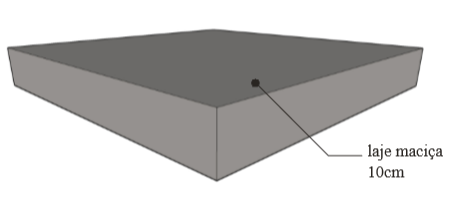
\includegraphics[width=0.4\textwidth]{figures/tab11-fig4.png}}  &                                                                       &                                                               & \multirow{5}{*}{\makecell[l]{Laje maciça \footnotesize(10 cm);\\ Sem telhamento.}}                                                                                                                         \\
                                                                                    &                                                                       &                                                               &                                                                                                                                                                                               \\
                                                                                    & 3,73                                                                  & 220                                                           &                                                                                                                                                                                               \\
                                                                                    &                                                                       &                                                               &                                                                                                                                                                                               \\
                                                                                    &                                                                       &                                                               &                                                                                                                                                                                               \\
                                                                                    &                                                                       &                                                               &                                                                                                                                                                                               \\ \hline
    \multicolumn{4}{c}{\textbf{Continua}}                                                                                                                                                                                                                                                                                                                                                                                   \\ \hline
\end{tabular}
\end{table} \pagebreak

\begin{table}[]
    \small
    \begin{tabular*}{\columnwidth}{@{\extracolsep{\fill}}lccl}
    \hline
    \multicolumn{4}{c}{\textbf{Conclusão}}                                                                                                                                                                                                                                                                                                                                                                                                  \\ \hline
    \multirow{9}{*}{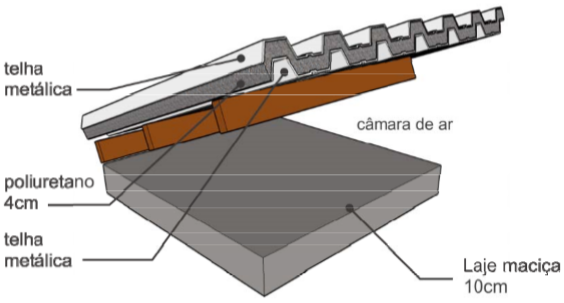
\includegraphics[width=0.4\textwidth]{figures/tab11-fig5.png}}  &                                                                       &                                            & \multirow{9}{*}{\makecell[l]{Laje pré-moldada (12 cm) \\(concreto 4 cm + EPS 7 cm + \\argamassa (1 cm);\\ Câmara de ar (\textgreater 5,0 cm);\\ Telha metálica (0,1 cm);\\ Poliuretano (4,0 cm);\\ Telha metálica (0,1 cm).}}    \\
                                                                                    &                                                                       &                                            &                                                                                                                                                                                                                                  \\
                                                                                    &                                                                       &                                            &                                                                                                                                                                                                                                  \\
                                                                                    &                                                                       &                                            &                                                                                                                                                                                                                                  \\
                                                                                    & 0,55                                                                  & 230                                        &                                                                                                                                                                                                                                  \\
                                                                                    &                                                                       &                                            &                                                                                                                                                                                                                                  \\
                                                                                    &                                                                       &                                            &                                                                                                                                                                                                                                  \\
                                                                                    &                                                                       &                                            &                                                                                                                                                                                                                                  \\
                                                                                    &                                                                       &                                            &                                                                                                                                                                                                                                  \\ \hline
    \multirow{9}{*}{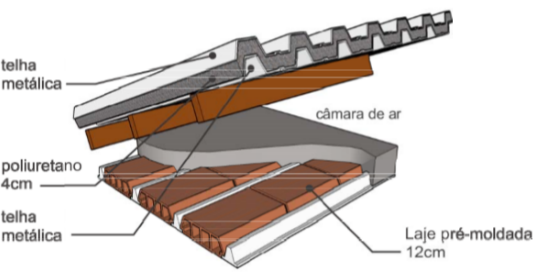
\includegraphics[width=0.4\textwidth]{figures/tab11-fig6.png}}  &                                                                       &                                            & \multirow{9}{*}{\makecell[l]{Laje maciça (10,0 cm);\\ Câmara de ar (\textgreater 5,0 cm);\\ Telha metálica (0,1 cm);\\ Poliestireno (isopor) (4,0 cm);\\ Telha metálica (0,1 cm).}}                                              \\
                                                                                    &                                                                       &                                            &                                                                                                                                                                                                                                  \\
                                                                                    &                                                                       &                                            &                                                                                                                                                                                                                                  \\
                                                                                    &                                                                       &                                            &                                                                                                                                                                                                                                  \\
                                                                                    & 0,53                                                                  & 176                                        &                                                                                                                                                                                                                                  \\
                                                                                    &                                                                       &                                            &                                                                                                                                                                                                                                  \\
                                                                                    &                                                                       &                                            &                                                                                                                                                                                                                                  \\
                                                                                    &                                                                       &                                            &                                                                                                                                                                                                                                  \\
                                                                                    &                                                                       &                                            &                                                                                                                                                                                                                                  \\ \hline
    \end{tabular*}
    \begin{flushleft}
        \par \small Fonte: autor (2019).\vspace{-0.6cm}
    \end{flushleft}
    \end{table}

\noindent A mudança de composição de vidro baseou-se na melhoria do desempenho energético para as zonas térmicas, onde a transmissão de radiação solar para o interior dos ambientes fosse mitigada, sem prejudicar o aproveitamento de luz natural \cite{CentroBrasileirodeEficienciaEnergeticaemEdificacoesCB3E2015,AssociacaoBrasileiradeNormasTecnicas-ABNT2013a,InstitutoNacionaldeMetrologiaNormalizacaoeQualidadeIndustrial-INMETRO2013,Ferreira2017} INSTITUTO..., 2013). Para tal, foi adotado o modelo mais eficiente, com baixa emissividade, como destacado na Tabela \ref{tab:tabela12}.
\begin{table}[H]
    \centering
    \small
    \caption{Propriedades físicas dos vidros adotados para os modelos genéricos.}
    \label{tab:tabela12}
    \begin{tabular}{lll}
    \hline
    \multicolumn{3}{c}{\textbf{Propriedade dos vidros}}                            \\ \hline
    \textbf{Fabricante}                      & CEBRACE          & CEBRACE          \\ \hline
    \textbf{Nome}                            & Reflecta Incolor & COOL-LITE ST 108 \\ \hline
    \textbf{Espessura}                       & 8 mm             & 6 mm             \\ \hline
    \textbf{Transmitância solar}             & 0,350            & 0,064            \\ \hline
    \textbf{Refletância solar externa (1)}   & 0,350            & 0,381            \\ \hline
    \textbf{Refletância visível interna (2)} & 0,340            & 0,485            \\ \hline
    \textbf{Transmitância visível}           & 0,320            & 0,078            \\ \hline
    \textbf{Refletância visível externa (1)} & 0,480            & 0,444            \\ \hline
    \textbf{Refletância visível interna (2)} & 0,510            & 0,377            \\ \hline
    \textbf{Emissividade externa (1)}        & 0,840            & 0,837            \\ \hline
    \textbf{Emissividade interna (2)}        & 0,840            & 0,147            \\ \hline
    \textbf{Condutividade}                   & 1,000            & 1,000            \\ \hline
    \textbf{Processo}                        & Laminado Incolor & Monolítico       \\ \hline
    \textbf{Transmitância ou U-value}        & 5,700            & 3,608            \\ \hline
    \textbf{Fator Solar ou SHGC}             & 0,440            & 0,160            \\ \hline
    \end{tabular}
    \begin{flushleft}
        \par \small Fonte: autor (2019).
    \end{flushleft}
    \end{table}
\vspace{-0.3cm} \noindent O PAF\textsubscript{T} foi implementado, variando entre 30\%, 50\% e 80\%, com a finalidade de evidenciar a influência sobre o consumo de energia relacionado às dimensões das aberturas e a área opaca das fachadas. Por relacionar componentes como a parede e o vidro, é um parâmetro de grande importância para o processo de determinação da eficiência energética.
\noindent Foram dimensionadas as proteções solares para cada um dos modelos, com base na incidência de orientação solar das edificações levantadas e no nível de obstrução vertical observado. Com o objetivo de bloquear a radiação solar direta presente nos horários mais quentes do dia, foram propostos brises fixos horizontais sobre as fachadas dos modelos genéricos entre os horários de 9 horas até às 16 horas. A escolha destes horários e a incidência de radiação solar direta é baseada em estudos de Hensen e Lamberts \citeyear{Hensen2012}.
\begin{figure}[H]
    \centering
    \caption{Detalhe da proteção solar de 1 m de comprimento da fachada oeste (a); carta solar da proteção solar de 1m (b)}
    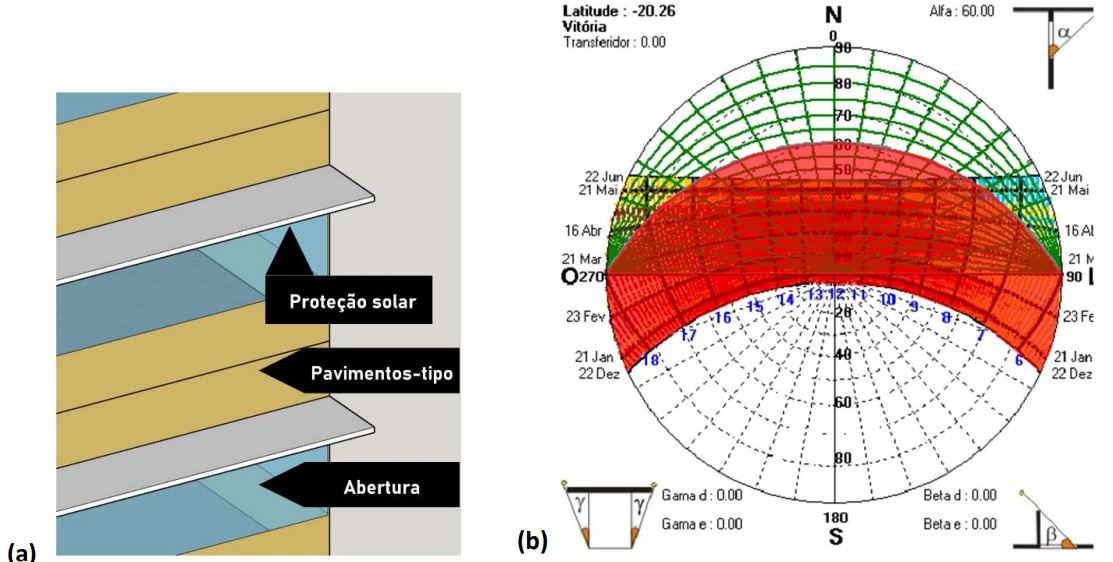
\includegraphics[width=1\textwidth]{figures/fig11-protecaosolar.jpg}
    \begin{flushleft}
        \par \small Fonte: autor (2019)
    \end{flushleft}
    \label{fig:figura12}
\end{figure}
\subsubsection{Volume e encadeamento das simulações}
\noindent Com a confirmação do número de parâmetros e variáveis necessários para a etapa de simulação, foi analisada a quantidade de interações entre as variáveis definidas. Esta análise visou apontar a viabilidade de execução do volume de simulação para a determinação da eficiência energética dos modelos com o aparato computacional disponível.\vspace*{0.3cm} \newline
\noindent Para tal, utilizou-se uma análise combinatória simples, onde foram combinados entre si os números de 9 parâmetros e 24 variáveis, como apresentado na Tabela \ref{tab:tabela9}. O resultado da análise, sem importância de ordem entre os elementos e sem repetição de ordem entre as variáveis, foi de 1.307.504 possibilidades de combinação. Considerando que a capacidade computacional disponível para a análise de todas essas possibilidades é limitada e que o tempo de simulação para cada possibilidade, neste trabalho tratada como cenário, é curto \cite{Werneck2017}, porém, dado o volume de cenários, torna-se impraticável dentro do tempo de desenvolvimento estipulado para a conclusão do trabalho.\vspace*{0.3cm} \newline
\noindent Dada a quantidade de combinações, optou-se pela fixação de 6 parâmetros, ou seja, sistemas de condicionamento de ar; medidas de redução de carga de energia de iluminação e equipamentos; transmitâncias de paredes, cobertura e proteção solar; e alteração de 3 parâmetros, de forma sequencial, sendo eles o PAF\textsubscript{T}; vidro; e a orientação solar, criando, assim, 192 cenários para cada modelo genérico, totalizando 384 cenários.\vspace*{0.3cm} \newline
\noindent A criação destes cenários tem como finalidade a redução do volume de simulações e evidenciar a influência das variáveis arquitetônicas sobre as edificações criadas. Baseado em ASHRAE et al. \citeyear{AmericanSocietyofHeatingRefrigeratingandAir-ConditioningEngineers-ASHRAE2019}, Costa \citeyear{Costa2018}, e Veloso \citeyear{Veloso2017}, os cenários foram segmentados em 10 blocos de simulação, segmentação esta apresentada pela Figura \ref{fig:figura13}. Os blocos de simulação com variáveis fixas representam as implementações incrementais de medida de redução de consumo de energia, enquanto os blocos com variáveis aleatórias são implementados em todos os cenários.\pagebreak
\begin{figure}[H]
    \centering
    \caption{Descrição simplificada dos blocos de simulação.}
    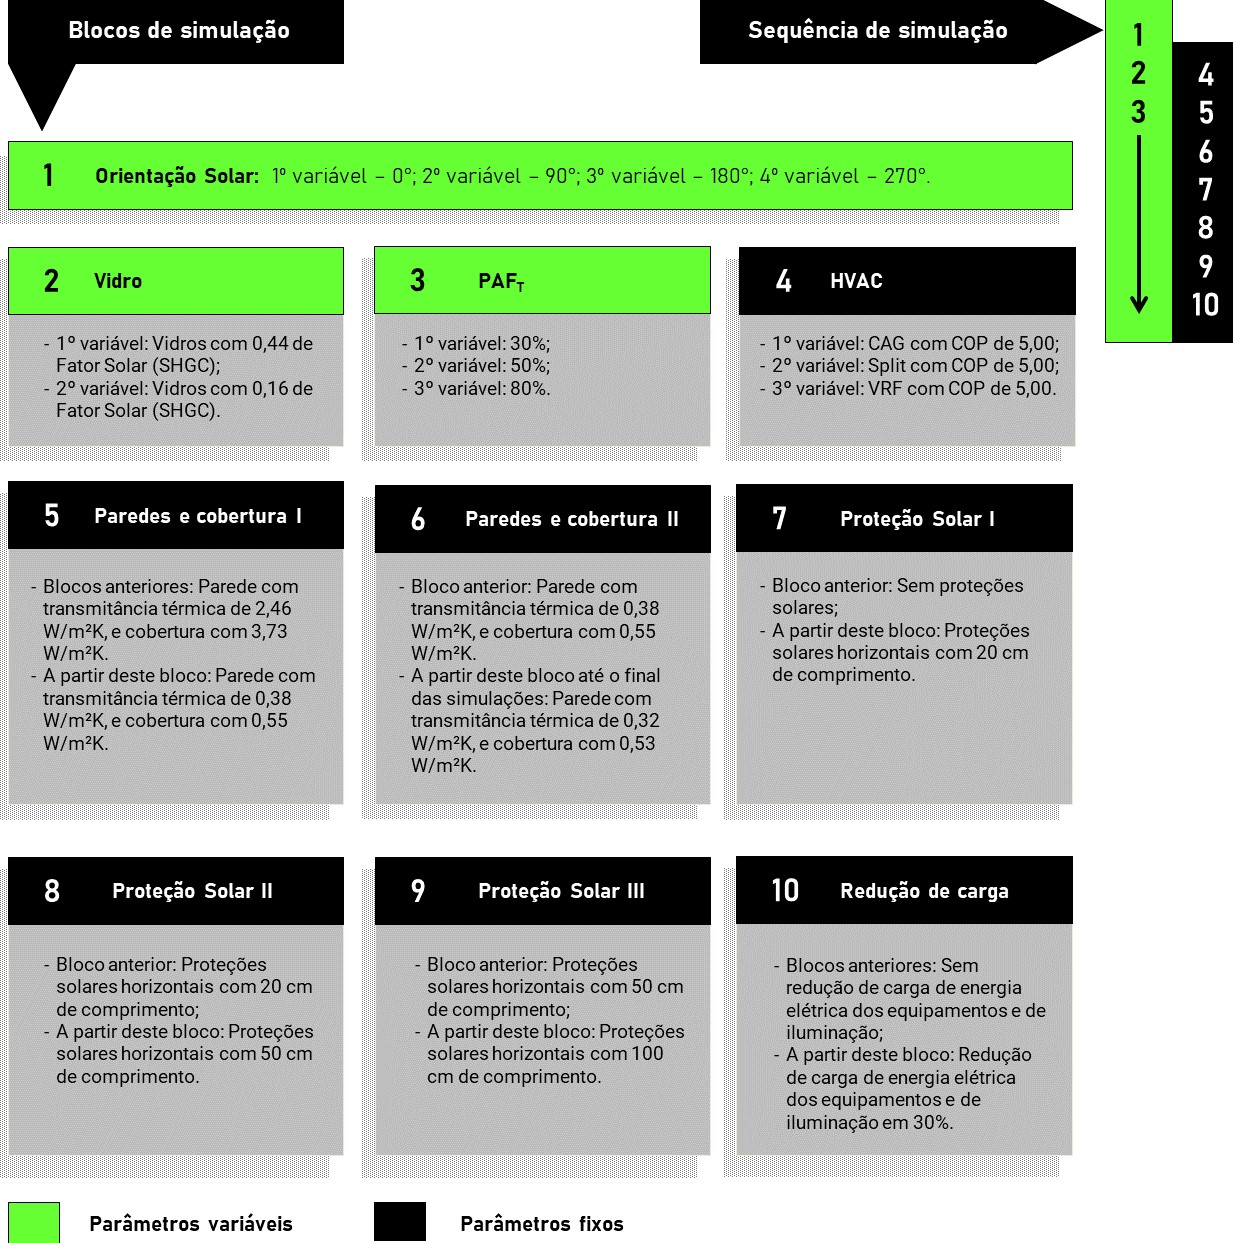
\includegraphics[width=1.0\textwidth]{figures/fig13-fluxograma.jpg}
    \begin{flushleft}
        \par \small Fonte: autor (2019)
    \end{flushleft}
    \label{fig:figura13}
\end{figure}
\noindent Tendo em vista os parâmetros apresentados na Tabela 10, os blocos de simulação são compostos por características básicas atribuídas para a envoltória, materiais e componentes, sistemas de condicionamento de ar, iluminação e equipamentos, características estas representadas pelas variáveis “a”. Da mesma forma, as implementações de redução de consumo de energia são apresentadas pelas variáveis “b”, “c” e “d”.\vspace*{0.3cm} \newline
\noindent Do primeiro ao terceiro bloco de simulações, compostos por 32 cenários, foram variadas as características de orientação solar, vidros e PAF\textsubscript{T} das edificações propostas. Concomitante à implementação do bloco de simulação 2, o sistema de condicionamento de ar “a”, sistema presente no levantamento, foi substituído pela opção “b”, sistema mais eficiente proposto. Deste ponto em diante, os blocos 4 a 10 foram implementados sequencialmente aos blocos de simulação 1 a 3. Todavia, as variáveis foram analisadas isoladamente cujas análises encontram-se relatadas no capítulo sobre o impacto das variáveis sobre o consumo anual de energia elétrica.\vspace*{0.3cm} \newline
\noindent Após os blocos 1 a 3 iniciados, foram inseridos, ao longo da sequência de simulações, os 7 blocos de simulação com variáveis fixas, compostos por 24 cenários cada. Estes blocos são compostos por sistemas de condicionamento de ar, alteração dos parâmetros de composição construtiva de paredes e cobertura, inserção de proteções solares e medidas de redução de consumo de carga de energia elétrica para equipamentos e iluminação. Estas variáveis fixas foram implementadas de forma incremental e sequencial, de acordo com a finalização da simulação precedente, a fim de evidenciar a influência de cada medida sobre o consumo energético.\vspace*{0.3cm} \newline
\noindent Com a conclusão do encadeamento de sequência das simulações, pôde-se desenvolver o processo de modelagem dedicado aos blocos de simulação.